\documentclass[dvips]{beamer}
%\documentclass[handout]{beamer}

\usepackage{pgf,pgfarrows,pgfnodes,pgfautomata,pgfheaps}
\mode<handout>
{
	\usepackage{pgfpages}	
	\pgfpagesuselayout{4 on 1}[a4paper,landscape,border shrink=5mm]
	%\pgfpagesuselayout{2 on 1}[a4paper,portrait,border shrink=5mm]
}
\mode<trans>
{
	\usepackage{pgfpages}	
	\pgfpagesuselayout{4 on 1}[a4paper,landscape,border shrink=5mm]
	%\pgfpagesuselayout{2 on 1}[a4paper,portrait,border shrink=5mm]
}

\usepackage{pstricks}
\usepackage{etex}
%\usepackage{beamerThemeGccTutorial}
\usepackage{beamerThemeGccWorkshop}
\usepackage{colortbl}
\usepackage{pst-node}
\usepackage{pst-grad}
\usepackage{pst-text}
\usepackage{pst-rel-points}
\usepackage{amssymb}
\usepackage{epsfig}
\usepackage{calc}
\usepackage{ifthen}
\usepackage{mydefs}
\usepackage{rotating}
\usepackage{multido}
\usepackage{multirow}
\usepackage[normalem]{ulem}
\usepackage{hyperref}

\newrgbcolor  {lightbrown}   {.65  0.45   0.4}

%\renewcommand{\large}{\normalsize}
\newcommand{\NULL}{\mbox{\sf\em NULL\/}}
\newcommand{\ul}[1]{{\blue #1}}
\newcommand{\myuparrow}{\mbox{$\uparrow$}}
\newcommand{\myarrow}{\mbox{\psset{unit=1mm}\psset{arrowsize=2}\psset{linewidth=.5}%
        \begin{pspicture}(-.25,-2)(4.,0)\psline{->}(0,-.75)(3.75,-.75)\end{pspicture}}}

\setbeamercolor{normal text}{fg=black,bg=white}
\newcommand{\blk}{\setbeamercolor{structure}{fg=blue!90!black,bg=white}}
\newcommand{\high}{\setbeamercolor{alerted text}{fg=blue!90!black,bg=blue!20!black}}
%
%
\setbeamersize{text margin left=15pt}
\setbeamersize{text margin right=15pt}
\setbeamersize{sidebar width right=0pt}
\setbeamersize{sidebar width left=0pt}
%\setbeamercolor{structure}{fg=black,bg=gray!40!white}
\setbeamercolor{frametitle}{fg=red}
\setbeamercolor{footline}{fg=brown}
\setbeamercolor{headline}{fg=brown}
\setbeamerfont{title}{shape=\itshape}
\setbeamerfont{frametitle}{series=\bfseries}
\setbeamercolor{title}{bg=white,fg=blue}
\setbeamercolor{author}{fg=brown}
\setbeamerfont{date}{size=\footnotesize}
\setbeamerfont{shortdate}{size=\footnotesize}
\setbeamerfont{part page}{size=\huge,shape=\itshape}

\title[Global Value Numbering]{Global Value Numbering}
\author[Kartik Singhal]{Kartik Singhal}
\institute[CSED, NIT Calicut ]{Department of Computer Science and Engineering\\ 
National Institute of Technology Calicut}
\titlegraphic{\scalebox{.4}{
\includegraphics[width=0.30\textwidth]{nitc-logo.eps}}}
\date[Nov 7, 2012]{Wednesday November 7, 2012}

\listfiles

%%%%%%%%%%%%% Yellow
\newrgbcolor{yel}{0.95 1 .8}
\newcmykcolor{lightyellow}{0 0 .3 0}
\newcmykcolor{llyellow}{0 0 .2 .1}
%%%%%%%%%%%%% Green
\newrgbcolor{darkgreen}{0 .5 0}
%%%%%%%%%%%%% Gray
\newgray{lightgray}{.85}
\newgray{dgray}{.35}
\newgray{ldgray}{.75}
%%%%%%%%%%%%% Pink
\newcmykcolor{lpink}{0 .2 0 0}
\newrgbcolor{pink}{1 .5 .6}
%%%%%%%%%%%%% Magenta
\newcmykcolor{lmagenta}{0 .4 0 0}
%%%%%%%%%%%%% Blue
\newrgbcolor{oldlightblue}{.1 .85 1}
\newrgbcolor{lightblue}{.75 0.85 1}
\newrgbcolor{newlightblue}{.75 0.75 1}
\newrgbcolor{myblueother}{.5 .5 1}
\newrgbcolor{myblue}{.15 .15 .8}
\newrgbcolor{darkblue}{0 0 .5}
\newcmykcolor{llblue}{.2 .15 0 .1}
\newcmykcolor{lblue}{.3 .2 0 .1}
%%%%%%%%%%%%% Brown
\newrgbcolor{brown}{.65 0.15 .0}
%%%%%%%%%%%%% Cream
\newrgbcolor{cream}{.95 0.95 .65}
%%%%%%%%%%%%% Violet
\newrgbcolor{violet}{.84 0 .96}
\newrgbcolor{mygreen}{.24 .84 .72}
\definecolor{paleturquoise}{RGB}{175 238 238}
\newrgbcolor{aquablue}{.4 .84 .86}
\definecolor{turquoise}{RGB}{64 224 208}
\definecolor{teal}{RGB}{0 128 128}
\newrgbcolor{lightblue}{.75 0.85 1}
%%%%%%%%%%%%% Green
\definecolor{darkgreen}{RGB}{0 50 0}
\definecolor{springreen}{RGB}{0 250 154}
\definecolor{greenyellow}{RGB}{152 250 152}
%%%%%%%%%%%% Brown
\definecolor{blanchedalmond}{RGB}{255 222 173}
%%%%%%%%%%%%% Yellow
\newrgbcolor{yel}{0.95 1 .8}
\newcmykcolor{lightyellow}{0 0 .3 0}
\newcmykcolor{llyellow}{0 0 .2 .1}
%%%%%%%%%%%%% Green
\newrgbcolor{darkgreen}{0 .5 0}
%%%%%%%%%%%%% Gray
\newgray{lightgray}{.85}
\newgray{dgray}{.35}
\newgray{ldgray}{.75}
%%%%%%%%%%%%% Pink
\newcmykcolor{lpink}{0 .2 0 0}
\newrgbcolor{pink}{1 .5 .6}
%%%%%%%%%%%%% Magenta
\newcmykcolor{lmagenta}{0 .4 0 0}
%%%%%%%%%%%%% Blue
\newrgbcolor{oldlightblue}{.1 .85 1}
\newrgbcolor{lightblue}{.75 0.85 1}
\newrgbcolor{newlightblue}{.75 0.75 1}
\newrgbcolor{myblueother}{.5 .5 1}
\newrgbcolor{myblue}{.15 .15 .8}
\newrgbcolor{darkblue}{0 0 .5}
\newcmykcolor{llblue}{.2 .15 0 .1}
\newcmykcolor{lblue}{.3 .2 0 .1}
%%%%%%%%%%%%% Brown
\newrgbcolor{brown}{.65 0.15 .0}
%%%%%%%%%%%%% Cream
\newrgbcolor{cream}{.95 0.95 .65}
%%%%%%%%%%%%% Violet
\newrgbcolor{violet}{.84 0 .96}
\newrgbcolor{mygreen}{.24 .84 .72}
\newcommand{\irulethree}{\rule{0cm}{.3cm}}
\newcommand{\irulefour}{\rule{0cm}{.4cm}}
\newcommand{\irulefive}{\rule{0cm}{.5cm}}
\newcommand{\irulesix}{\rule{0cm}{.6cm}}


\newcommand{\lptr}{\mbox{\bfseries\footnotesize lptr}}
\newcommand{\rptr}{\mbox{\bfseries\footnotesize rptr}}
%\includeonlyframes{current}

\newcommand{\notesPage}{
\psset{unit=1mm}
\begin{pspicture}(0,0)(120,80)
\rput{90}(0,40){\scalebox{1}{\Huge\bfseries\gray Notes}}
\end{pspicture}
}

\begin{document}

\frame[plain]{
\only<1|trans:1|handout:1>{
\titlepage
}
\only<0|trans:2|handout:0>{
}
}
\part{Outline}

\addtocounter{part}{-1}


\frame{
\frametitle{Outline}

\only<1|trans:1|handout:1>{
\begin{itemize}
\setlength{\itemsep}{2mm}
\item Problem Definition
\item Introduction
\begin{itemize}
\item GVN
\item Some Known Algorithms
\item Motivation
\end{itemize}
\item Work Done
\begin{itemize}
\item Compiler Infrastructures
\item Structure of GCC
\item Intermediate Forms
\item Work Flow
\item A Na\"{\i}ve Implementation of Constant Propagation
\end{itemize}
\item Conclusion \& Future Work
\item References
\end{itemize}
}
\only<presentation:0|trans:2|handout:0>{
\notesPage
}
}

%\input{par-vect-theory}
\part{\protect\parbox{3.75in}{\protect\centering Problem Definition}}
\frame[plain]{
\only<1|trans:1|handout:1>{\partpage}
\only<presentation:0|trans:2|handout:0>{
\notesPage
}
}

\addtocounter{part}{-1}
\psset{unit=1mm}

\part{Problem Definition}

\frame{
\frametitle{Problem Definition}
\only<1|trans:1|handout:1>{
To {\color{red}study global value numbering, a compiler optimization, in detail}; to review and compare known algorithms; to implement one of the best among them; and in the process, improve upon the algorithm if possible.
}
\only<0|trans:2|handout:0>{
\notesPage
}
}

\frame{
\frametitle{Problem Definition}
\only<1|trans:1|handout:1>{
To study global value numbering, a compiler optimization, in detail; {\color{red}to review and compare known algorithms}; to implement one of the best among them; and in the process, improve upon the algorithm if possible.
}
\only<0|trans:2|handout:0>{
\notesPage
}
}

\frame{
\frametitle{Problem Definition}
\only<1|trans:1|handout:1>{
To study global value numbering, a compiler optimization, in detail; to review and compare known algorithms; {\color{red}to implement one of the best among them}; and in the process, improve upon the algorithm if possible.
}
\only<0|trans:2|handout:0>{
\notesPage
}
}

\frame{
\frametitle{Problem Definition}
\only<1|trans:1|handout:1>{
To study global value numbering, a compiler optimization, in detail; to review and compare known algorithms; to implement one of the best among them; {\color{red}and in the process, improve upon the algorithm if possible}.
}
\only<0|trans:2|handout:0>{
\notesPage
}
}


%\input{par-vect-theory}
\part{\protect\parbox{3.75in}{\protect\centering Introduction}}
\frame[plain]{
\only<1|trans:1|handout:1>{\partpage}
\only<presentation:0|trans:2|handout:0>{
\notesPage
}
}

\addtocounter{part}{-1}
\psset{unit=1mm}

\part{Introduction}


\newcommand{\cell}[1]{\psframe[fillcolor=#1,fillstyle=solid,linestyle=none](0,0)(10,10)}
\newcommand{\mycolorbox}[3]{\psframebox*[fillstyle=solid,fillcolor=#1]{\makebox[#2]{\rule{0mm}{#2}\protect#3}}}


\newcommand{\gline}{{\protect\psline[linecolor=black,arrowsize=1.5mm,arrowinset=0]{*->}(1,1)(7.25,10.25)}}
 \newcommand{\bline}{{\protect\psline[linecolor=blue,arrowsize=1.5mm,arrowinset=0]{*->}(1,1)(7.25,10.25)}}
  \newcommand{\rcurveselfloop}{{\protect\pscurve[linecolor=red,arrowsize=1.5mm,arrowinset=0]{*->}(1,1)(1.75,3.5)(1,5.5)(0,6)(-1,5.5)(-1.75,3.5)(-1.5,.5)}}
\newcommand{\gcurveselfloop}{{\protect\pscurve[linecolor=black,arrowsize=1.5mm,arrowinset=0]{*->}(1,1)(1.75,3.5)(1,5.5)(0,6)(-1,5.5)(-1.75,3.5)(-1.5,.5)}}
\newcommand{\glinestraight}{{\protect\psline[linecolor=black,arrowsize=1.5mm,arrowinset=0]{*->}(0,1)(0,10)}}
 \newcommand{\blinestraight}{{\protect\psline[linecolor=blue,arrowsize=1.5mm,arrowinset=0]{*->}(0,1)(0,10)}}
  \newcommand{\rcurve}{{\protect\pscurve[linecolor=red,arrowsize=1.5mm,arrowinset=0]{*->}(-1.5,1)(-1.5,3.5)(-3.75,6)(-5.5,4.5)(-6,0)}}
\newcommand{\gcurve}{{\protect\pscurve[linecolor=black,arrowsize=1.5mm,arrowinset=0]{*->}(-1.5,1)(-1.5,3.5)(-3.75,6)(-5.5,4.5)(-6,0)}}
  \newcommand{\rcurveforward}{{\protect\pscurve[linecolor=red,arrowsize=1.5mm,arrowinset=0]{<-*}(0,0)(-.5,4.5)(-2.25,6)(-4.25,3.5)(-4.5,1)}}
\newcommand{\gcurveforward}{{\protect\pscurve[linecolor=black,arrowsize=1.5mm,arrowinset=0]{<-*}(0,0)(-.5,4.5)(-2.25,6)(-4.25,3.5)(-4.5,1)}}
\newcommand{\Loc}{\text{$m$}}
\newcommand{\flowd}{\text{\rule{0em}{1em}$\delta$}}
\newcommand{\antid}{\text{\rule{0em}{1.1em}$\bar{\delta}$}}
\newcommand{\outd}{\text{\rule{0em}{1.1em}$\delta^O$}}

\frame{
\frametitle{GVN}
\only<1|trans:1|handout:1>{
Global value numbering (GVN) is a program analysis that categorizes expressions in the program that compute the same value. This information
can be used to remove redundant computations.
}
\only<0|trans:2|handout:0>{
\notesPage
}
}

\frame{
\frametitle{Some Known Algorithms}
\only<1|trans:1|handout:1>{

\begin{description}
  \item[Kildall '73] \hfill \\
  Introduced a precise global analysis algorithm for program optimization by using the concept of an optimizing function for generalization.
  \item[AWZ '88] \hfill \\
  Introduced an efficient algorithm, uses a value graph to represent symbolic execution of program. Represents the values of variables after a join using a selection
function $\phi$, as in SSA, treats them as uninterpreted, hence remains incomplete.
\end{description}

}
\only<0|trans:2|handout:0>{
\notesPage
}
}

\frame{
\frametitle{Some Known Algorithms}
\only<1|trans:1|handout:1>{

\begin{description}
  \item[RKS '99] \hfill \\
  Introduced polynomial time algorithm, extended the algorithm by AWZ. Employs a normalization process using some rewrite rules for terms involving $\phi$ functions, until congruence classes reach a fixed point. More
equivalances, optimal for acyclic programs but remains incomplete.
  \item[Gargi '02] \hfill \\
  Proposed balanced algorithms, extends AWZ to perform forward propagation and reassociation and to consider back edges in SSA graph. Discovers more equivalences but is still incomplete.
  \item[Gulwani '04] \hfill \\
  Proposed a polynomial time algorithm which is optimal if only equalities of bounded size are considered.
\end{description}

}
\only<0|trans:2|handout:0>{
\notesPage
}
}

\frame{
\frametitle{Motivation}
\only<1|trans:1|handout:1>{

\begin{itemize}
\item A compiler is a fairly large software program and forms an excellent software engineering case study.
\item Optimizing compilers are hard to build.
\item Study of compiler optimizations provides a good blend of theory (for generality and correctness) and practice (for validation and efficiency).
\item Global Value Numbering, specifically, is an interesting global dataflow analysis for study.
\item Opportunity to work on a popular open souce project's code base.
\end{itemize}

}
\only<0|trans:2|handout:0>{
\notesPage
}
}

\frame{
\frametitle{Motivation}
\only<1|trans:1|handout:1>{

And \ldots
\begin{figure}
\centering{
{\includegraphics[width=0.70\textwidth]{grc.eps}}
\\
{Essential Abstractions in GCC `12 - A workshop on GCC Internals by GCC Resource Center, IIT Bombay.}
}
\end{figure}

}
\only<0|trans:2|handout:0>{
\notesPage
}
}

%\input{par-vect-theory}
\part{\protect\parbox{3.75in}{\protect\centering Work Done}}
\frame[plain]{
\only<1|trans:1|handout:1>{\partpage}
\only<presentation:0|trans:2|handout:0>{
\notesPage
}
}

\addtocounter{part}{-1}
\psset{unit=1mm}

\part{Work Done}

\frame{
\frametitle{Compiler Infrastructures}
\only<1|trans:1|handout:1>{

\begin{itemize}
  \item SUIF - Stanford University Intermediate Format
  \item GCC - GNU Compiler Collection
  \item LLVM
\end{itemize}

We choose GCC as our implementation platform as it is a popular, professional, open-source compiler and could yield more realistic results.

}
\only<0|trans:2|handout:0>{
\notesPage
}
}

\frame{
\frametitle{Structure of GCC}
\only<1|trans:1|handout:1>{

Conceptually three phases:

\begin{enumerate}
\item There is a separate front end for each supported language. A front end takes the source code, translates that source code into a semantically equivalent, language independent abstract syntax tree (AST). The syntax and semantics of this AST are defined by the GIMPLE language, the highest level language independent intermediate representation GCC has.
\end{enumerate}
}
\only<0|trans:2|handout:0>{
\notesPage
}
}

\frame{
\frametitle{Structure of GCC}
\only<1|trans:1|handout:1>{

Conceptually three phases:

\begin{enumerate}
\setcounter{enumi}{1}
\item This AST is then run through a list of target independent code transformations that take care of constructing a control flow graph, and optimizing the AST for optimizing compilations, lowering to non-strict RTL (expand), and running RTL based optimizations for optimizing compilations. The non-strict RTL is handed over to more low-level passes.
\end{enumerate}

}
\only<0|trans:2|handout:0>{
\notesPage
}
}

\frame{
\frametitle{Structure of GCC}
\only<1|trans:1|handout:1>{

Conceptually three phases:

\begin{enumerate}
\setcounter{enumi}{2}
\item The low-level passes are the passes that are part of the code generation process. The first job of these passes is to turn the non-strict RTL representation into strict RTL. Other jobs of the strict RTL passes include scheduling, doing peephole optimizations, and emitting the assembly output.
\end{enumerate}

}
\only<0|trans:2|handout:0>{
\notesPage
}
}

\frame{
\frametitle{Intermediate Forms}
\only<1|trans:1|handout:1>{

\begin{figure}
\centering{
{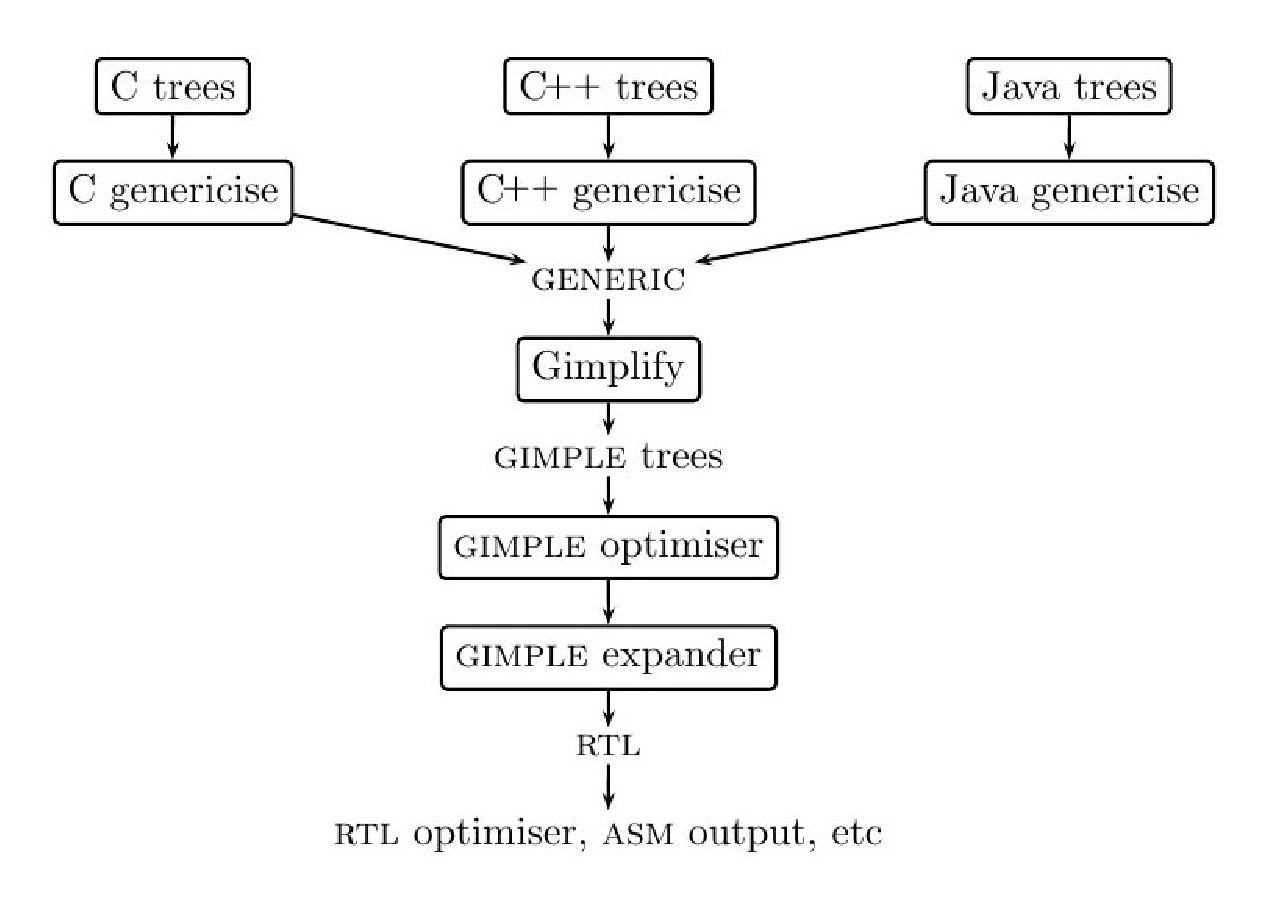
\includegraphics[width=0.60\textwidth]{./ir2-framework.eps}}
\\
{IR Framework in GCC}
}
\end{figure}

We work on GIMPLE which is a three-address intermediate form.
}
\only<0|trans:2|handout:0>{
\notesPage
}
}

\frame{
\frametitle{Workflow}
\only<1|trans:1|handout:1>{

\begin{figure}
\centering{
{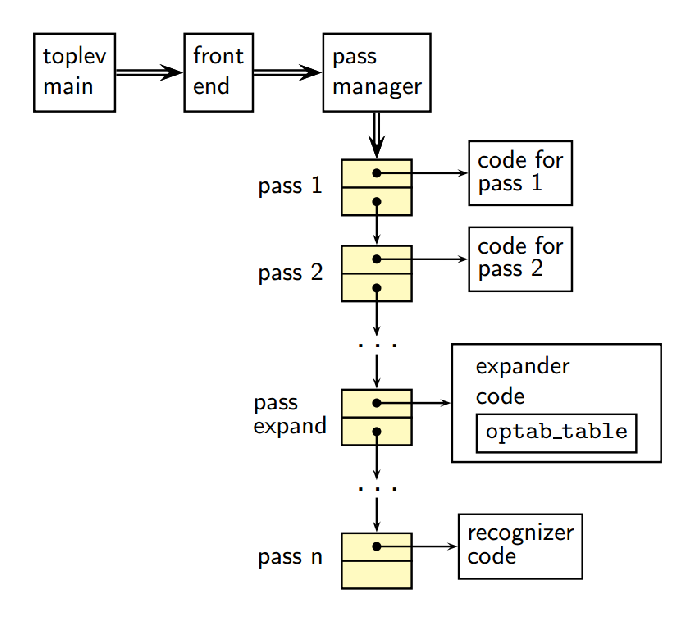
\includegraphics[width=0.50\textwidth]{./plugin1.eps}}
\\
{Plugin Structure in GCC}
}
\end{figure}

}
\only<0|trans:2|handout:0>{
\notesPage
}
}

\frame{
\frametitle{Workflow}
\only<1|trans:1|handout:1>{

\begin{figure}
\centering{
{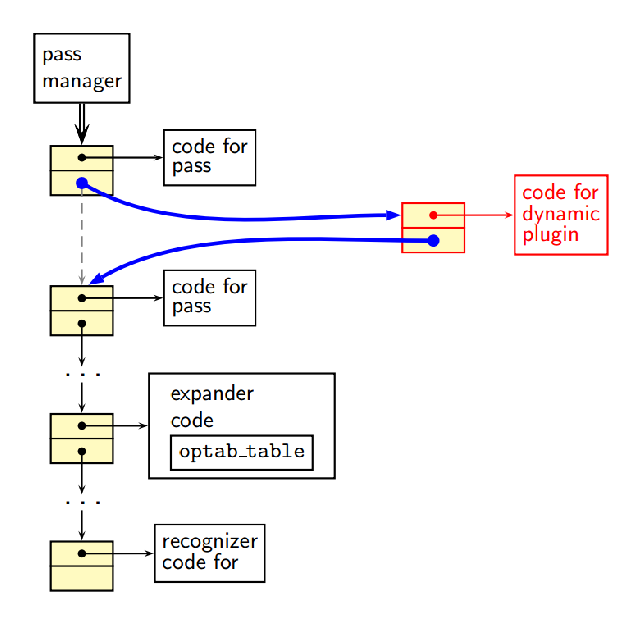
\includegraphics[width=0.50\textwidth]{./dynamic-plugin1.eps}}
\\
{Dynamic Plugin Mechanism in GCC}
}
\end{figure}

}
\only<0|trans:2|handout:0>{
\notesPage
}
}

\frame{
\frametitle{A Na\"{\i}ve Implementation of Constant Propagation}
\only<1|trans:1|handout:1>{

\begin{figure}
\centering{
{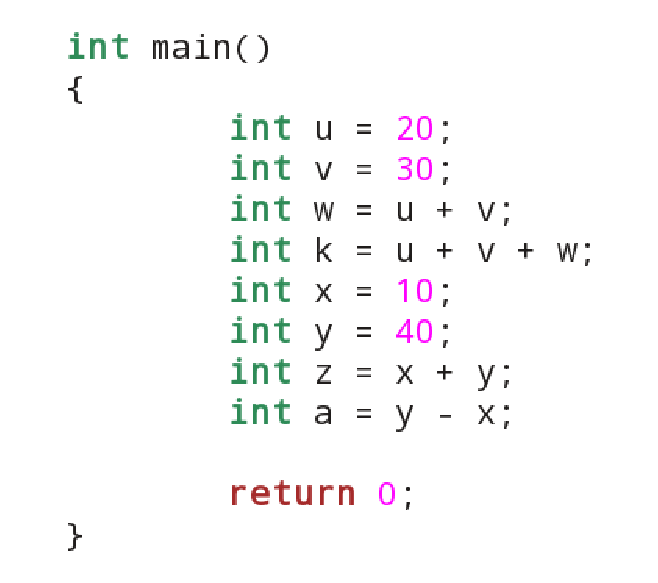
\includegraphics[width=0.30\textwidth]{./test.eps}}
\\
{Test program in C}
}
\end{figure}

}
\only<0|trans:2|handout:0>{
\notesPage
}
}

\frame{
\frametitle{A Na\"{\i}ve Implementation of Constant Propagation}
\only<1|trans:1|handout:1>{

\begin{figure}
\centering{
{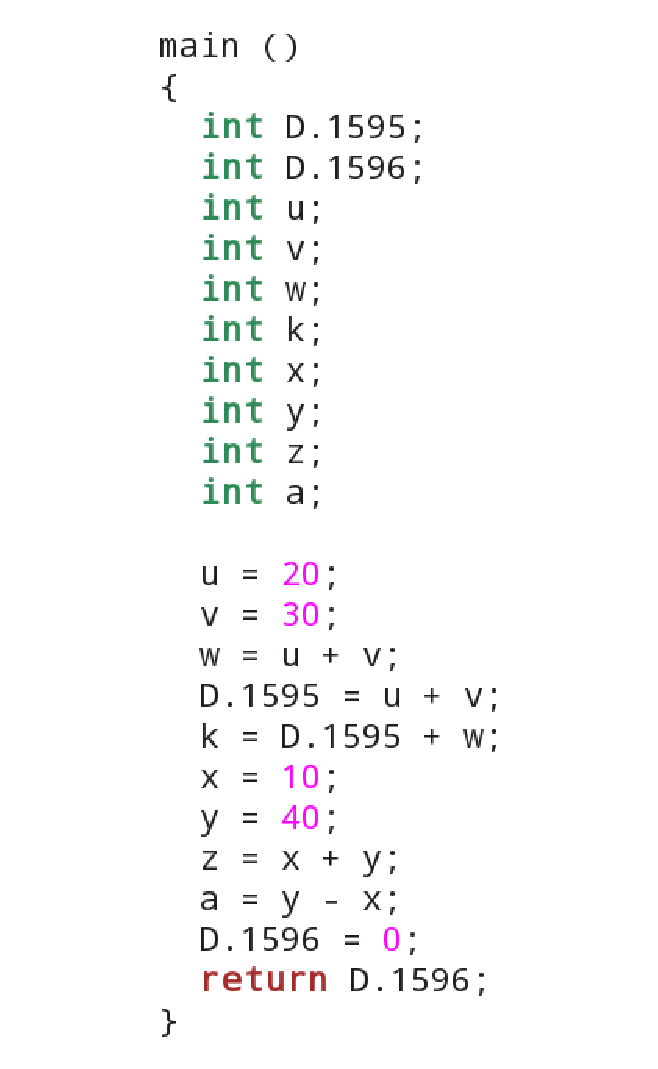
\includegraphics[width=0.30\textwidth]{./gimple.eps}}
\\
{In GIMPLE IR form}
}
\end{figure}

}
\only<0|trans:2|handout:0>{
\notesPage
}
}

\frame{
\frametitle{A Na\"{\i}ve Implementation of Constant Propagation}
\only<1|trans:1|handout:1>{

\begin{figure}
\centering{
{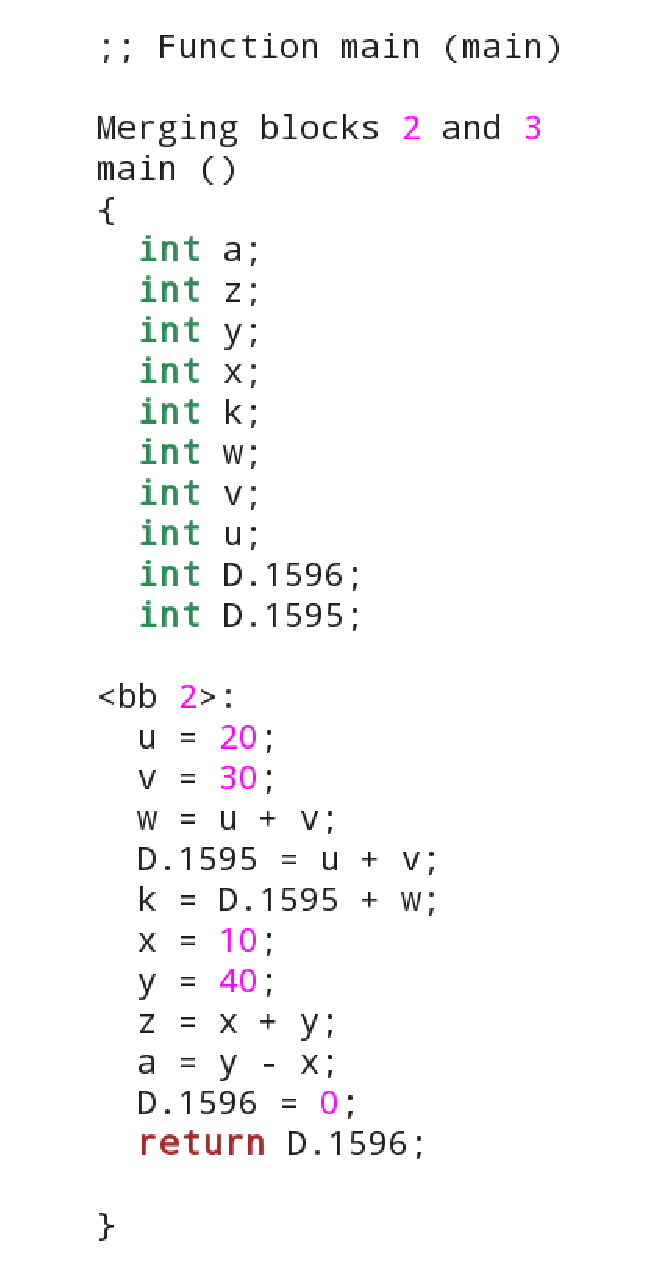
\includegraphics[width=0.30\textwidth]{./cfg.eps}}
\\
{After CFG pass}
}
\end{figure}

}
\only<0|trans:2|handout:0>{
\notesPage
}
}

\frame{
\frametitle{A Na\"{\i}ve Implementation of Constant Propagation}
\only<1|trans:1|handout:1>{

\begin{figure}
\centering{
{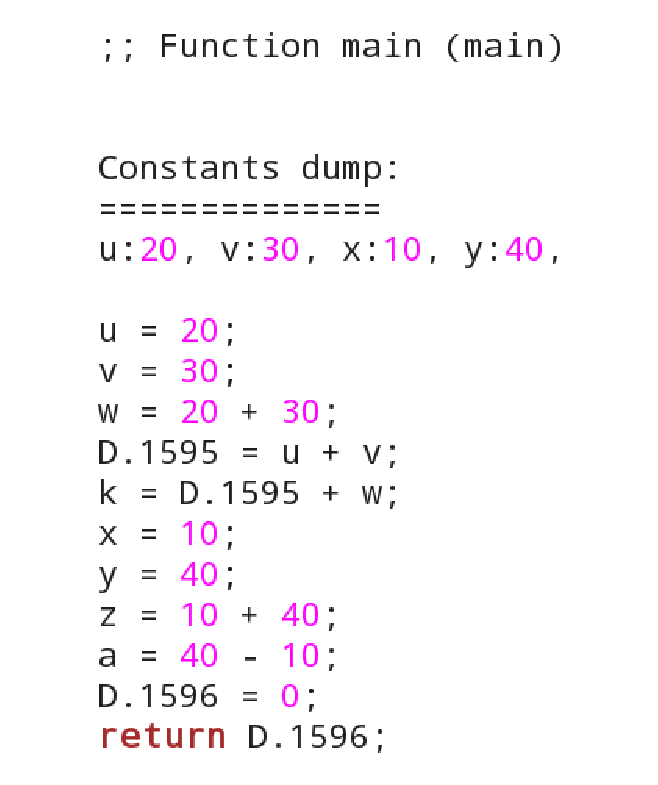
\includegraphics[width=0.30\textwidth]{./const.eps}}
\\
{Dump produced by our plugin}
}
\end{figure}

}
\only<0|trans:2|handout:0>{
\notesPage
}
}

%\input{par-vect-theory}
\part{\protect\parbox{3.75in}{\protect\centering Conclusion \& Future Work}}
\frame[plain]{
\only<1|trans:1|handout:1>{\partpage}
\only<presentation:0|trans:2|handout:0>{
\notesPage
}
}

\addtocounter{part}{-1}
\psset{unit=1mm}

\part{Conclusion \& Future Work}

\frame{
\frametitle{Conclusion \& Future Work}
\only<1|trans:1|handout:1>{
Pros and cons of a number of known value numbering algorithms have been
evaluated and familiarity with functionality of GCC as a compiler research
infrastructure gained.\\[0.8cm]

We plan to use GCC for implementation of a global value numbering algorithm, test and compare its performance with other known algorithms and
look for any possible improvements in the algorithm during the remaining course of the project.

}
\only<0|trans:2|handout:0>{
\notesPage
}
}


%\input{par-vect-theory}
\part{\protect\parbox{3.75in}{\protect\centering References}}
\frame[plain]{
\only<1|trans:1|handout:1>{\partpage}
\only<presentation:0|trans:2|handout:0>{
\notesPage
}
}

\addtocounter{part}{-1}
\psset{unit=1mm}

\part{References}

\frame{
\frametitle{References}
\only<1|trans:1|handout:1>{
\begin{itemize}
\item Gary A. Kildall. 1973. A unified approach to global program optimization. In \emph{Proceedings of the 1st annual ACM SIGACT-SIGPLAN symposium on Principles of programming languages} (POPL '73). ACM, 194-206.\ \url{http://doi.acm.org/10.1145/512927.512945}
\item B. Alpern, M. N. Wegman, and F. K. Zadeck. 1988. Detecting equality of variables in programs. In \emph{Proceedings of the 15th ACM SIGPLAN-SIGACT symposium on Principles of programming languages} (POPL '88). ACM, 1-11.\ \url{http://doi.acm.org/10.1145/73560.73561}
\item R\"uthing, O., Knoop, J., \& Steffen, B. 1999. Detecting equalities of variables: Combining efficiency with precision. \emph{Static Analysis}, 848-848.
\end{itemize}
}
\only<0|trans:2|handout:0>{
\notesPage
}
}

\frame{
\frametitle{References}
\only<1|trans:1|handout:1>{
\begin{itemize}
\item Karthik Gargi. 2002. A sparse algorithm for predicated global value numbering. In \emph{Proceedings of the ACM SIGPLAN 2002 Conference on Programming language design and implementation} (PLDI '02). ACM, 45-56.\ \url{http://doi.acm.org/10.1145/512529.512536}
\item Gulwani, S., \& Necula, G. 2004. A polynomial-time algorithm for global value numbering. \emph{Static Analysis}, 703-1020.
\item VanDrunen, T. J. 2004. Partial redundancy elimination for global value numbering (Doctoral dissertation, Purdue University).
\item Essential Abstractions in GCC '12 - A workshop on GCC Internals by GCC Resource Center, IIT Bombay.\ \url{http://www.cse.iitb.ac.in/grc/gcc-workshop-12}
\item Structure of GCC -\ \url{http://gcc.gnu.org/wiki/StructureOfGCC}
\end{itemize}
}
\only<0|trans:2|handout:0>{
\notesPage
}
}

\addtocounter{part}{-1}
\psset{unit=1mm}

\part{Thanks}


\frame{
\frametitle{}
\only<1|trans:1|handout:1>{

\centering{\Huge{Thank You}}

}
\only<0|trans:2|handout:0>{
\notesPage
}
}

\end{document}
